% Options for packages loaded elsewhere
\PassOptionsToPackage{unicode}{hyperref}
\PassOptionsToPackage{hyphens}{url}
%
\documentclass[
]{article}
\usepackage{amsmath,amssymb}
\usepackage{iftex}
\ifPDFTeX
  \usepackage[T1]{fontenc}
  \usepackage[utf8]{inputenc}
  \usepackage{textcomp} % provide euro and other symbols
\else % if luatex or xetex
  \usepackage{unicode-math} % this also loads fontspec
  \defaultfontfeatures{Scale=MatchLowercase}
  \defaultfontfeatures[\rmfamily]{Ligatures=TeX,Scale=1}
\fi
\usepackage{lmodern}
\ifPDFTeX\else
  % xetex/luatex font selection
\fi
% Use upquote if available, for straight quotes in verbatim environments
\IfFileExists{upquote.sty}{\usepackage{upquote}}{}
\IfFileExists{microtype.sty}{% use microtype if available
  \usepackage[]{microtype}
  \UseMicrotypeSet[protrusion]{basicmath} % disable protrusion for tt fonts
}{}
\makeatletter
\@ifundefined{KOMAClassName}{% if non-KOMA class
  \IfFileExists{parskip.sty}{%
    \usepackage{parskip}
  }{% else
    \setlength{\parindent}{0pt}
    \setlength{\parskip}{6pt plus 2pt minus 1pt}}
}{% if KOMA class
  \KOMAoptions{parskip=half}}
\makeatother
\usepackage{xcolor}
\usepackage{color}
\usepackage{fancyvrb}
\newcommand{\VerbBar}{|}
\newcommand{\VERB}{\Verb[commandchars=\\\{\}]}
\DefineVerbatimEnvironment{Highlighting}{Verbatim}{commandchars=\\\{\}}
% Add ',fontsize=\small' for more characters per line
\newenvironment{Shaded}{}{}
\newcommand{\AlertTok}[1]{\textcolor[rgb]{1.00,0.00,0.00}{\textbf{#1}}}
\newcommand{\AnnotationTok}[1]{\textcolor[rgb]{0.38,0.63,0.69}{\textbf{\textit{#1}}}}
\newcommand{\AttributeTok}[1]{\textcolor[rgb]{0.49,0.56,0.16}{#1}}
\newcommand{\BaseNTok}[1]{\textcolor[rgb]{0.25,0.63,0.44}{#1}}
\newcommand{\BuiltInTok}[1]{\textcolor[rgb]{0.00,0.50,0.00}{#1}}
\newcommand{\CharTok}[1]{\textcolor[rgb]{0.25,0.44,0.63}{#1}}
\newcommand{\CommentTok}[1]{\textcolor[rgb]{0.38,0.63,0.69}{\textit{#1}}}
\newcommand{\CommentVarTok}[1]{\textcolor[rgb]{0.38,0.63,0.69}{\textbf{\textit{#1}}}}
\newcommand{\ConstantTok}[1]{\textcolor[rgb]{0.53,0.00,0.00}{#1}}
\newcommand{\ControlFlowTok}[1]{\textcolor[rgb]{0.00,0.44,0.13}{\textbf{#1}}}
\newcommand{\DataTypeTok}[1]{\textcolor[rgb]{0.56,0.13,0.00}{#1}}
\newcommand{\DecValTok}[1]{\textcolor[rgb]{0.25,0.63,0.44}{#1}}
\newcommand{\DocumentationTok}[1]{\textcolor[rgb]{0.73,0.13,0.13}{\textit{#1}}}
\newcommand{\ErrorTok}[1]{\textcolor[rgb]{1.00,0.00,0.00}{\textbf{#1}}}
\newcommand{\ExtensionTok}[1]{#1}
\newcommand{\FloatTok}[1]{\textcolor[rgb]{0.25,0.63,0.44}{#1}}
\newcommand{\FunctionTok}[1]{\textcolor[rgb]{0.02,0.16,0.49}{#1}}
\newcommand{\ImportTok}[1]{\textcolor[rgb]{0.00,0.50,0.00}{\textbf{#1}}}
\newcommand{\InformationTok}[1]{\textcolor[rgb]{0.38,0.63,0.69}{\textbf{\textit{#1}}}}
\newcommand{\KeywordTok}[1]{\textcolor[rgb]{0.00,0.44,0.13}{\textbf{#1}}}
\newcommand{\NormalTok}[1]{#1}
\newcommand{\OperatorTok}[1]{\textcolor[rgb]{0.40,0.40,0.40}{#1}}
\newcommand{\OtherTok}[1]{\textcolor[rgb]{0.00,0.44,0.13}{#1}}
\newcommand{\PreprocessorTok}[1]{\textcolor[rgb]{0.74,0.48,0.00}{#1}}
\newcommand{\RegionMarkerTok}[1]{#1}
\newcommand{\SpecialCharTok}[1]{\textcolor[rgb]{0.25,0.44,0.63}{#1}}
\newcommand{\SpecialStringTok}[1]{\textcolor[rgb]{0.73,0.40,0.53}{#1}}
\newcommand{\StringTok}[1]{\textcolor[rgb]{0.25,0.44,0.63}{#1}}
\newcommand{\VariableTok}[1]{\textcolor[rgb]{0.10,0.09,0.49}{#1}}
\newcommand{\VerbatimStringTok}[1]{\textcolor[rgb]{0.25,0.44,0.63}{#1}}
\newcommand{\WarningTok}[1]{\textcolor[rgb]{0.38,0.63,0.69}{\textbf{\textit{#1}}}}
\usepackage{graphicx}
\makeatletter
\def\maxwidth{\ifdim\Gin@nat@width>\linewidth\linewidth\else\Gin@nat@width\fi}
\def\maxheight{\ifdim\Gin@nat@height>\textheight\textheight\else\Gin@nat@height\fi}
\makeatother
% Scale images if necessary, so that they will not overflow the page
% margins by default, and it is still possible to overwrite the defaults
% using explicit options in \includegraphics[width, height, ...]{}
\setkeys{Gin}{width=\maxwidth,height=\maxheight,keepaspectratio}
% Set default figure placement to htbp
\makeatletter
\def\fps@figure{htbp}
\makeatother
\setlength{\emergencystretch}{3em} % prevent overfull lines
\providecommand{\tightlist}{%
  \setlength{\itemsep}{0pt}\setlength{\parskip}{0pt}}
\setcounter{secnumdepth}{-\maxdimen} % remove section numbering
\ifLuaTeX
  \usepackage{selnolig}  % disable illegal ligatures
\fi
\IfFileExists{bookmark.sty}{\usepackage{bookmark}}{\usepackage{hyperref}}
\IfFileExists{xurl.sty}{\usepackage{xurl}}{} % add URL line breaks if available
\urlstyle{same}
\hypersetup{
  hidelinks,
  pdfcreator={LaTeX via pandoc}}

\author{}
\date{}

\begin{document}

\section{Cutting-plane Method and Its Amazing
Oracles}\label{cutting-plane-method-and-its-amazing-oracles}

@luk036

2022-11-03

\begin{center}\rule{0.5\linewidth}{0.5pt}\end{center}

class: middle, right

\begin{quote}
When you have eliminated the impossible, whatever remains, however
improbable, must be the truth.
\end{quote}

\emph{Sir Arthur Conan Doyle, stated by Sherlock Holmes}

\begin{center}\rule{0.5\linewidth}{0.5pt}\end{center}

class: middle, center

\section{Introduction}\label{introduction}

\begin{center}\rule{0.5\linewidth}{0.5pt}\end{center}

\subsection{Common Perspective of Ellipsoid
Method}\label{common-perspective-of-ellipsoid-method}

\begin{itemize}
\item
  It is widely believed to be inefficient in practice for large-scale
  problems.

  \begin{itemize}
  \item
    Convergent rate is slow, even when using deep cuts.
  \item
    Cannot exploit sparsity.
  \end{itemize}
\item
  It has since then supplanted by the interior-point methods.
\item
  Used only as a theoretical tool to prove polynomial-time solvability
  of some combinatorial optimization problems.
\end{itemize}

\begin{center}\rule{0.5\linewidth}{0.5pt}\end{center}

\subsection{But\ldots{}}\label{but}

\begin{itemize}
\item
  The ellipsoid method works very differently compared with the interior
  point methods.
\item
  Only require a \emph{separation oracle}. Can play nicely with other
  techniques.
\item
  While the ellipsoid method itself cannot take advantage of sparsity,
  the oracle can.
\end{itemize}

\begin{center}\rule{0.5\linewidth}{0.5pt}\end{center}

\subsection{Consider the ellipsoid method
when\ldots{}}\label{consider-the-ellipsoid-method-when}

\begin{itemize}
\item
  The number of optimization variables is moderate, e.g.~ECO flow,
  analog circuit sizing, parametric problems
\item
  The number of constraints is large, or even infinite
\item
  Oracle can be implemented effectively.
\end{itemize}

\begin{center}\rule{0.5\linewidth}{0.5pt}\end{center}

class: middle, center

\section{Cutting-plane Method
Revisited}\label{cutting-plane-method-revisited}

\begin{center}\rule{0.5\linewidth}{0.5pt}\end{center}

\subsection{Convex Set}\label{convex-set}

.pull-left70{[}

\begin{itemize}
\tightlist
\item
  Let \(\mathcal{K} \subseteq \mathbb{R}^n\) be a convex set.
\item
  Consider the feasibility problem:

  \begin{itemize}
  \tightlist
  \item
    Find a point \(x^* \in \mathbb{R}^n\) in \(\mathcal{K}\),
  \item
    or determine that \(\mathcal{K}\) is empty (i.e., there is no
    feasible solution)
  \end{itemize}
\end{itemize}

{]} .pull-right30{[}

\begin{figure}
\centering

\includegraphics{ellipsoid.files/region.pdf}
\caption{image}
\end{figure}

{]}

\begin{center}\rule{0.5\linewidth}{0.5pt}\end{center}

\subsection{Separation Oracle}\label{separation-oracle}

.pull-left70{[}

\begin{itemize}
\tightlist
\item
  When a separation oracle \(\Omega\) is \emph{queried} at \(x_0\), it
  either

  \begin{itemize}
  \tightlist
  \item
    asserts that \(x_0 \in \mathcal{K}\), or
  \item
    returns a separating hyperplane between \(x_0\) and \(\mathcal{K}\):
    \[g^\mathsf{T} (x - x_0) + \beta \le 0, \beta \geq 0, g \neq 0, \;
          \forall x \in \mathcal{K}\]
  \end{itemize}
\end{itemize}

{]} .pull-right30{[}

\begin{figure}
\centering
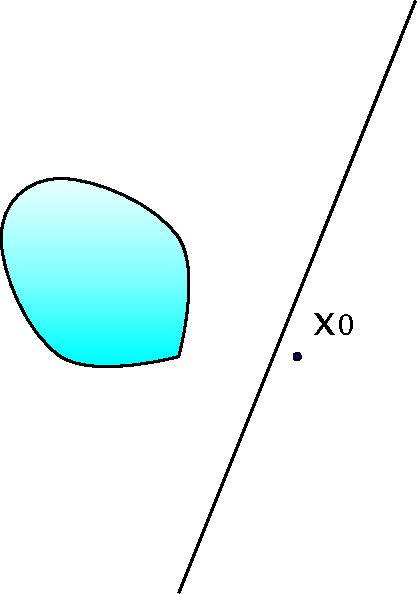
\includegraphics{ellipsoid.files/cut.pdf}
\caption{image}
\end{figure}

{]}

\begin{center}\rule{0.5\linewidth}{0.5pt}\end{center}

\subsection{Separation Oracle (cont'd)}\label{separation-oracle-contd}

\begin{itemize}
\item
  \((g, \beta)\) is called a \emph{cutting-plane}, or cut, because it
  eliminates the half-space
  \(\{x \mid g^\mathsf{T} (x - x_0) + \beta > 0\}\) from our search.
\item
  If \(\beta=0\) (\(x_0\) is on the boundary of halfspace that is cut),
  the cutting-plane is called \emph{neutral cut}.
\item
  If \(\beta>0\) (\(x_0\) lies in the interior of halfspace that is
  cut), the cutting-plane is called \emph{deep cut}.
\item
  If \(\beta<0\) (\(x_0\) lies in the exterior of halfspace that is
  cut), the cutting-plane is called \emph{shallow cut}.
\end{itemize}

\begin{center}\rule{0.5\linewidth}{0.5pt}\end{center}

\subsection{Subgradient}\label{subgradient}

\begin{itemize}
\item
  \(\mathcal{K}\) is usually given by a set of inequalities
  \(f_j(x) \le 0\) or \(f_j(x) < 0\) for \(j = 1 \cdots m\), where
  \(f_j(x)\) is a convex function.
\item
  A vector \(g \equiv \partial f(x_0)\) is called a subgradient of a
  convex function \(f\) at \(x_0\) if
  \(f(z) \geq f(x_0) + g^\mathsf{T} (z - x_0)\).
\item
  Hence, the cut \((g, \beta)\) is given by
  \((\partial f(x_0), f(x_0))\)
\end{itemize}

Remarks:

\begin{itemize}
\tightlist
\item
  If \(f(x)\) is differentiable, we can simply take
  \(\partial f(x_0) = \nabla f(x_0)\)
\end{itemize}

\begin{center}\rule{0.5\linewidth}{0.5pt}\end{center}

\subsection{Key components of Cutting-plane
method}\label{key-components-of-cutting-plane-method}

\begin{itemize}
\tightlist
\item
  A cutting plane oracle \(\Omega\)
\item
  A search space \(\mathcal{S}\) initially large enough to cover
  \(\mathcal{K}\), e.g.

  \begin{itemize}
  \tightlist
  \item
    Polyhedron \(\mathcal{P}\) = \(\{z \mid C z \preceq d \}\)
  \item
    Interval \(\mathcal{I}\) = \([l, u]\) (for one-dimensional problem)
  \item
    Ellipsoid \(\mathcal{E}\) =
    \(\{z \mid (z-x_c)P^{-1}(z-x_c) \le 1 \}\)
  \end{itemize}
\end{itemize}

\begin{center}\rule{0.5\linewidth}{0.5pt}\end{center}

\subsection{Generic Cutting-plane
method}\label{generic-cutting-plane-method}

\begin{itemize}
\tightlist
\item
  \textbf{Given} initial \(\mathcal{S}\) known to contain
  \(\mathcal{K}\).
\item
  \textbf{Repeat}

  \begin{enumerate}
  \def\labelenumi{\arabic{enumi}.}
  \tightlist
  \item
    Choose a point \(x_0\) in \(\mathcal{S}\)
  \item
    Query the cutting-plane oracle at \(x_0\)
  \item
    \textbf{If} \(x_0 \in \mathcal{K}\), quit
  \item
    \textbf{Else}, update \(\mathcal{S}\) to a smaller set that covers:
    \[\mathcal{S}^+ = \mathcal{S} \cap \{z \mid g^\mathsf{T} (z - x_0) + \beta \le 0\}\]
  \item
    \textbf{If} \(\mathcal{S}^+ = \emptyset\) or it is small enough,
    quit.
  \end{enumerate}
\end{itemize}

\begin{center}\rule{0.5\linewidth}{0.5pt}\end{center}

\subsection{Corresponding Python code}\label{corresponding-python-code}

\begin{Shaded}
\begin{Highlighting}[]
\KeywordTok{def}\NormalTok{ cutting\_plane\_feas(omega, S, options}\OperatorTok{=}\NormalTok{Options()):}
    \ControlFlowTok{for}\NormalTok{ niter }\KeywordTok{in} \BuiltInTok{range}\NormalTok{(options.max\_iter):}
\NormalTok{        cut }\OperatorTok{=}\NormalTok{ omega.assess\_feas(S.xc)  }\CommentTok{\# query the oracle at S.xc}
        \ControlFlowTok{if}\NormalTok{ cut }\KeywordTok{is} \VariableTok{None}\NormalTok{:  }\CommentTok{\# feasible sol\textquotesingle{}n obtained}
            \ControlFlowTok{return} \VariableTok{True}\NormalTok{, niter, CutStatus.Success}
\NormalTok{        cutstatus, tsq }\OperatorTok{=}\NormalTok{ S.update(cut)  }\CommentTok{\# update S}
        \ControlFlowTok{if}\NormalTok{ cutstatus }\OperatorTok{!=}\NormalTok{ CutStatus.Success:}
            \ControlFlowTok{return} \VariableTok{False}\NormalTok{, niter, cutstatus}
        \ControlFlowTok{if}\NormalTok{ tsq }\OperatorTok{\textless{}}\NormalTok{ options.tol:}
            \ControlFlowTok{return} \VariableTok{False}\NormalTok{, niter, CutStatus.SmallEnough}
    \ControlFlowTok{return} \VariableTok{False}\NormalTok{, options.max\_iter, CutStatus.NoSoln}
\end{Highlighting}
\end{Shaded}

\begin{center}\rule{0.5\linewidth}{0.5pt}\end{center}

\subsection{From Feasibility to
Optimization}\label{from-feasibility-to-optimization}

\[\begin{array}{ll}
    \text{minimize}     & f_0(x), \\
    \text{subject to}   & x \in \mathcal{K}
\end{array}\]

\begin{itemize}
\item
  The optimization problem is treated as a feasibility problem with an
  additional constraint \(f_0(x) \le t\).
\item
  \(f_0(x)\) could be a convex or a \emph{quasiconvex function}.
\item
  \(t\) is also called the \emph{best-so-far} value of \(f_0(x)\).
\end{itemize}

\begin{center}\rule{0.5\linewidth}{0.5pt}\end{center}

\subsection{Convex Optimization
Problem}\label{convex-optimization-problem}

\begin{itemize}
\item
  Consider the following general form: \[\begin{array}{ll}
    \text{minimize}     & t, \\
    \text{subject to}   & \Phi(x, t) \le 0, \\
    & x \in \mathcal{K},
  \end{array}\] where \(\mathcal{K}'_t = \{x \mid \Phi(x, t) \le 0\}\)
  is the \(t\)-sublevel set of \(\{x \mid f_0(x) \le t\}\).
\item
  Note: \(\mathcal{K'}_t \subseteq \mathcal{K'}_u\) if and only if
  \(t \le u\) (monotonicity)
\item
  One easy way to solve the optimization problem is to apply the binary
  search on \(t\).
\end{itemize}

\begin{center}\rule{0.5\linewidth}{0.5pt}\end{center}

\begin{Shaded}
\begin{Highlighting}[]
\KeywordTok{def}\NormalTok{ bsearch(omega, intrvl, options}\OperatorTok{=}\NormalTok{Options()):}
    \CommentTok{\# assume monotone}
\NormalTok{    lower, upper }\OperatorTok{=}\NormalTok{ intrvl}
\NormalTok{    T }\OperatorTok{=} \BuiltInTok{type}\NormalTok{(upper)  }\CommentTok{\# T could be \textasciigrave{}int\textasciigrave{}}
    \ControlFlowTok{for}\NormalTok{ niter }\KeywordTok{in} \BuiltInTok{range}\NormalTok{(options.max\_iter):}
\NormalTok{        tau }\OperatorTok{=}\NormalTok{ (upper }\OperatorTok{{-}}\NormalTok{ lower) }\OperatorTok{/} \DecValTok{2}
        \ControlFlowTok{if}\NormalTok{ tau }\OperatorTok{\textless{}}\NormalTok{ options.tol:}
            \ControlFlowTok{return}\NormalTok{ upper, niter, CutStatus.SmallEnough}
\NormalTok{        t }\OperatorTok{=}\NormalTok{ T(lower }\OperatorTok{+}\NormalTok{ tau)}
        \ControlFlowTok{if}\NormalTok{ omega.assess\_bs(t):  }\CommentTok{\# feasible sol\textquotesingle{}n obtained}
\NormalTok{            upper }\OperatorTok{=}\NormalTok{ t}
        \ControlFlowTok{else}\NormalTok{:}
\NormalTok{            lower }\OperatorTok{=}\NormalTok{ t}
    \ControlFlowTok{return}\NormalTok{ upper, options.max\_iter, CutStatus.Unknown}
\end{Highlighting}
\end{Shaded}

\begin{center}\rule{0.5\linewidth}{0.5pt}\end{center}

\begin{Shaded}
\begin{Highlighting}[]
\KeywordTok{class}\NormalTok{ bsearch\_adaptor:}
    \KeywordTok{def} \FunctionTok{\_\_init\_\_}\NormalTok{(}\VariableTok{self}\NormalTok{, P, S, options}\OperatorTok{=}\NormalTok{Options()):}
        \VariableTok{self}\NormalTok{.P }\OperatorTok{=}\NormalTok{ P}
        \VariableTok{self}\NormalTok{.S }\OperatorTok{=}\NormalTok{ S}
        \VariableTok{self}\NormalTok{.options }\OperatorTok{=}\NormalTok{ options}

    \AttributeTok{@property}
    \KeywordTok{def}\NormalTok{ x\_best(}\VariableTok{self}\NormalTok{):}
        \ControlFlowTok{return} \VariableTok{self}\NormalTok{.S.xc}

    \KeywordTok{def}\NormalTok{ assess\_bs(}\VariableTok{self}\NormalTok{, t):}
\NormalTok{        S }\OperatorTok{=} \VariableTok{self}\NormalTok{.S.copy()}
        \VariableTok{self}\NormalTok{.P.update(t)}
\NormalTok{        ell\_info }\OperatorTok{=}\NormalTok{ cutting\_plane\_feas(}\VariableTok{self}\NormalTok{.P, S, }\VariableTok{self}\NormalTok{.options)}
        \ControlFlowTok{if}\NormalTok{ ell\_info.feasible:}
            \VariableTok{self}\NormalTok{.S.xc }\OperatorTok{=}\NormalTok{ S.xc}
        \ControlFlowTok{return}\NormalTok{ ell\_info.feasible}
\end{Highlighting}
\end{Shaded}

\begin{center}\rule{0.5\linewidth}{0.5pt}\end{center}

\subsection{Shrinking}\label{shrinking}

\begin{itemize}
\item
  Another possible way is, to update the best-so-far \(t\) whenever a
  feasible solution \(x'\) is found by solving the equation:
  \[\Phi(x', t_\text{new}) = 0 \, .\]
\item
  If the equation is difficuit to solve but \(t\) is also convex w.r.t.
  \(\Phi\), then we may create a new varaible, say \(z\) and let
  \(z \le t\).
\end{itemize}

\begin{center}\rule{0.5\linewidth}{0.5pt}\end{center}

\subsection{Generic Cutting-plane method
(Optim)}\label{generic-cutting-plane-method-optim}

\begin{itemize}
\tightlist
\item
  \textbf{Given} initial \(\mathcal{S}\) known to contain
  \(\mathcal{K}_t\).
\item
  \textbf{Repeat}

  \begin{enumerate}
  \def\labelenumi{\arabic{enumi}.}
  \tightlist
  \item
    Choose a point \(x_0\) in \(\mathcal{S}\)
  \item
    Query the separation oracle at \(x_0\)
  \item
    \textbf{If} \(x_0 \in \mathcal{K}_t\), update \(t\) such that
    \(\Phi(x_0, t) = 0\).
  \item
    Update \(\mathcal{S}\) to a smaller set that covers:
    \[\mathcal{S}^+ = \mathcal{S} \cap \{z \mid g^\mathsf{T} (z - x_0) + \beta \le 0\} \]
  \item
    \textbf{If} \(\mathcal{S}^+ = \emptyset\) or it is small enough,
    quit.
  \end{enumerate}
\end{itemize}

\begin{center}\rule{0.5\linewidth}{0.5pt}\end{center}

\begin{Shaded}
\begin{Highlighting}[]
\KeywordTok{def}\NormalTok{ cutting\_plane\_optim(omega, S, t, options}\OperatorTok{=}\NormalTok{Options()):}
\NormalTok{    x\_best }\OperatorTok{=} \VariableTok{None}
    \ControlFlowTok{for}\NormalTok{ niter }\KeywordTok{in} \BuiltInTok{range}\NormalTok{(options.max\_iter):}
\NormalTok{        cut, t1 }\OperatorTok{=}\NormalTok{ omega.assess\_optim(S.xc, t)}
        \ControlFlowTok{if}\NormalTok{ t1 }\KeywordTok{is} \KeywordTok{not} \VariableTok{None}\NormalTok{:  }\CommentTok{\# better t obtained}
\NormalTok{            t }\OperatorTok{=}\NormalTok{ t1}
\NormalTok{            x\_best }\OperatorTok{=}\NormalTok{ S.xc.copy()}
\NormalTok{        status, tsq }\OperatorTok{=}\NormalTok{ S.update(cut)}
        \ControlFlowTok{if}\NormalTok{ status }\OperatorTok{!=}\NormalTok{ CutStatus.Success:}
            \ControlFlowTok{return}\NormalTok{ x\_best, t, niter, status}
        \ControlFlowTok{if}\NormalTok{ tsq }\OperatorTok{\textless{}}\NormalTok{ options.tol:}
            \ControlFlowTok{return}\NormalTok{ x\_best, t, niter, CutStatus.SmallEnough}
    \ControlFlowTok{return}\NormalTok{ x\_best, t, options.max\_iter, CutStatus.Success}
\end{Highlighting}
\end{Shaded}

\begin{center}\rule{0.5\linewidth}{0.5pt}\end{center}

\subsection{Example - Profit Maximization
Problem}\label{example---profit-maximization-problem}

This example is taken from {[}@Aliabadi2013Robust{]}.

\[\begin{array}{ll}
   \text{maximize} & p(A x_1^\alpha x_2^\beta) - v_1 x_1 - v_2 x_2 \\
   \text{subject to}& x_1 \le k.
\end{array}\]

\begin{itemize}
\tightlist
\item
  \(p(A x_1^\alpha x_2^\beta)\) : Cobb-Douglas production function
\item
  \(p\): the market price per unit
\item
  \(A\): the scale of production
\item
  \(\alpha, \beta\): the output elasticities
\item
  \(x\): input quantity
\item
  \(v\): output price
\item
  \(k\): a given constant that restricts the quantity of \(x_1\)
\end{itemize}

\begin{center}\rule{0.5\linewidth}{0.5pt}\end{center}

\subsection{Example - Profit maximization
(cont'd)}\label{example---profit-maximization-contd}

\begin{itemize}
\tightlist
\item
  The formulation is not in the convex form.
\item
  Rewrite the problem in the following form: \[\begin{array}{ll}
    \text{maximize} & t \\
    \text{subject to} & t  + v_1 x_1  + v_2 x_2 \le p A x_1^{\alpha} x_2^{\beta}\\
                  & x_1 \le k.
    \end{array}\]
\end{itemize}

\begin{center}\rule{0.5\linewidth}{0.5pt}\end{center}

\subsection{Profit maximization in Convex
Form}\label{profit-maximization-in-convex-form}

\begin{itemize}
\item
  By taking the logarithm of each variable:

  \begin{itemize}
  \tightlist
  \item
    \(y_1 = \log x_1\), \(y_2 = \log x_2\).
  \end{itemize}
\item
  We have the problem in a convex form:
\end{itemize}

\[\begin{array}{ll}
    \text{max}  & t \\
    \text{s.t.} & \log(t + v_1 e^{y_1} + v_2 e^{y_2}) - (\alpha y_1 + \beta y_2) \le \log(pA) \\
                & y_1 \le \log k.
\end{array}\]

\begin{center}\rule{0.5\linewidth}{0.5pt}\end{center}

\begin{Shaded}
\begin{Highlighting}[]
\KeywordTok{class}\NormalTok{ ProfitOracle:}
    \KeywordTok{def} \FunctionTok{\_\_init\_\_}\NormalTok{(}\VariableTok{self}\NormalTok{, params, a, v):}
\NormalTok{        p, A, k }\OperatorTok{=}\NormalTok{ params}
        \VariableTok{self}\NormalTok{.log\_pA }\OperatorTok{=}\NormalTok{ np.log(p }\OperatorTok{*}\NormalTok{ A)}
        \VariableTok{self}\NormalTok{.log\_k }\OperatorTok{=}\NormalTok{ np.log(k)}
        \VariableTok{self}\NormalTok{.v }\OperatorTok{=}\NormalTok{ v}
        \VariableTok{self}\NormalTok{.a }\OperatorTok{=}\NormalTok{ a}

    \KeywordTok{def}\NormalTok{ assess\_optim(}\VariableTok{self}\NormalTok{, y, t):}
        \ControlFlowTok{if}\NormalTok{ (fj }\OperatorTok{:=}\NormalTok{ y[}\DecValTok{0}\NormalTok{] }\OperatorTok{{-}} \VariableTok{self}\NormalTok{.log\_k) }\OperatorTok{\textgreater{}} \FloatTok{0.0}\NormalTok{:  }\CommentTok{\# constraint}
\NormalTok{            g }\OperatorTok{=}\NormalTok{ np.array([}\FloatTok{1.0}\NormalTok{, }\FloatTok{0.0}\NormalTok{])}
            \ControlFlowTok{return}\NormalTok{ (g, fj), }\VariableTok{None}

\NormalTok{        log\_Cobb }\OperatorTok{=} \VariableTok{self}\NormalTok{.log\_pA }\OperatorTok{+} \VariableTok{self}\NormalTok{.a }\OperatorTok{@}\NormalTok{ y}
\NormalTok{        q }\OperatorTok{=} \VariableTok{self}\NormalTok{.v }\OperatorTok{*}\NormalTok{ np.exp(y)}
\NormalTok{        vx }\OperatorTok{=}\NormalTok{ q[}\DecValTok{0}\NormalTok{] }\OperatorTok{+}\NormalTok{ q[}\DecValTok{1}\NormalTok{]}
        \ControlFlowTok{if}\NormalTok{ (fj }\OperatorTok{:=}\NormalTok{ np.log(t }\OperatorTok{+}\NormalTok{ vx) }\OperatorTok{{-}}\NormalTok{ log\_Cobb) }\OperatorTok{\textgreater{}=} \FloatTok{0.0}\NormalTok{:}
\NormalTok{            g }\OperatorTok{=}\NormalTok{ q }\OperatorTok{/}\NormalTok{ (t }\OperatorTok{+}\NormalTok{ vx) }\OperatorTok{{-}} \VariableTok{self}\NormalTok{.a}
            \ControlFlowTok{return}\NormalTok{ (g, fj), }\VariableTok{None}

\NormalTok{        t }\OperatorTok{=}\NormalTok{ np.exp(log\_Cobb) }\OperatorTok{{-}}\NormalTok{ vx}
\NormalTok{        g }\OperatorTok{=}\NormalTok{ q }\OperatorTok{/}\NormalTok{ (t }\OperatorTok{+}\NormalTok{ vx) }\OperatorTok{{-}} \VariableTok{self}\NormalTok{.a}
        \ControlFlowTok{return}\NormalTok{ (g, }\FloatTok{0.0}\NormalTok{), t}
\end{Highlighting}
\end{Shaded}

\begin{center}\rule{0.5\linewidth}{0.5pt}\end{center}

\begin{Shaded}
\begin{Highlighting}[]
\CommentTok{\# Main program}

\ImportTok{import}\NormalTok{ numpy }\ImportTok{as}\NormalTok{ np}
\ImportTok{from}\NormalTok{ ellalgo.cutting\_plane }\ImportTok{import}\NormalTok{ cutting\_plane\_optim}
\ImportTok{from}\NormalTok{ ellalgo.ell }\ImportTok{import}\NormalTok{ Ell}
\ImportTok{from}\NormalTok{ ellalgo.oracles.profit\_oracle }\ImportTok{import}\NormalTok{ ProfitOracle}

\NormalTok{p, A, k }\OperatorTok{=} \FloatTok{20.0}\NormalTok{, }\FloatTok{40.0}\NormalTok{, }\FloatTok{30.5}
\NormalTok{params }\OperatorTok{=}\NormalTok{ p, A, k}
\NormalTok{alpha, beta }\OperatorTok{=} \FloatTok{0.1}\NormalTok{, }\FloatTok{0.4}
\NormalTok{v1, v2 }\OperatorTok{=} \FloatTok{10.0}\NormalTok{, }\FloatTok{35.0}
\NormalTok{a }\OperatorTok{=}\NormalTok{ np.array([alpha, beta])}
\NormalTok{v }\OperatorTok{=}\NormalTok{ np.array([v1, v2])}
\NormalTok{r }\OperatorTok{=}\NormalTok{ np.array([}\FloatTok{100.0}\NormalTok{, }\FloatTok{100.0}\NormalTok{])  }\CommentTok{\# initial ellipsoid (sphere)}

\NormalTok{E }\OperatorTok{=}\NormalTok{ Ell(r, np.array([}\FloatTok{0.0}\NormalTok{, }\FloatTok{0.0}\NormalTok{]))}
\NormalTok{P }\OperatorTok{=}\NormalTok{ ProfitOracle(params, a, v)}
\NormalTok{x, f, num\_iters, status }\OperatorTok{=}\NormalTok{ cutting\_plane\_optim(P, E, }\FloatTok{0.0}\NormalTok{)}
\ControlFlowTok{assert}\NormalTok{ x }\KeywordTok{is} \KeywordTok{not} \VariableTok{None}
\end{Highlighting}
\end{Shaded}

\begin{center}\rule{0.5\linewidth}{0.5pt}\end{center}

\subsection{Area of Applications}\label{area-of-applications}

\begin{itemize}
\tightlist
\item
  Robust convex optimization

  \begin{itemize}
  \tightlist
  \item
    oracle technique: affine arithmetic
  \end{itemize}
\item
  Parametric network potential problem

  \begin{itemize}
  \tightlist
  \item
    oracle technique: negative cycle detection
  \end{itemize}
\item
  Semidefinite programming

  \begin{itemize}
  \tightlist
  \item
    oracle technique: Cholesky or \(LDL^\mathsf{T}\) factorization
  \end{itemize}
\end{itemize}

\begin{center}\rule{0.5\linewidth}{0.5pt}\end{center}

class: middle, center

\section{Robust Convex Optimization}\label{robust-convex-optimization}

\begin{center}\rule{0.5\linewidth}{0.5pt}\end{center}

\subsection{Robust Optimization
Formulation}\label{robust-optimization-formulation}

\begin{itemize}
\item
  Consider: \[\begin{array}{ll}
    \text{minimize}   & \sup_{q \in \mathbb Q} f_0(x,q), \\
    \text{subject to} & f_j(x,q) \leq 0, \;
     \forall q \in {\mathbb Q}, \; j = 1,2,\cdots,m,
  \end{array}\] where \(q\) represents a set of varying parameters.
\item
  The problem can be reformulated as: \[\begin{array}{ll}
    \text{minimize}   & t \\
    \text{subject to} & f_0(x,q) < t  \\
    & f_j(x,q) \leq 0, \;
     \forall q \in {\mathbb Q}, \; j = 1,2,\cdots,m.
  \end{array}\]
\end{itemize}

\begin{center}\rule{0.5\linewidth}{0.5pt}\end{center}

\subsection{Example - Profit Maximization Problem
(convex)}\label{example---profit-maximization-problem-convex}

\[\begin{array}{ll}
\text{max}  & t \\
\text{s.t.} & \log(t + \hat{v}_1 e^{y_1} + \hat{v}_2 e^{y_2}) - (\hat{\alpha} y_1 + \hat{\beta} y_2) \le \log(\hat{p}\,A)  \\
                  & y_1 \le \log \hat{k} ,
\end{array}\]

\begin{itemize}
\tightlist
\item
  Now assume that:

  \begin{itemize}
  \tightlist
  \item
    \(\hat{\alpha}\) and \(\hat{\beta}\) vary \(\bar{\alpha} \pm e_1\)
    and \(\bar{\beta} \pm e_2\) respectively.
  \item
    \(\hat{p}\), \(\hat{k}\), \(\hat{v}_1\), and \(\hat{v}_2\) all vary
    \(\pm e_3\).
  \end{itemize}
\end{itemize}

\begin{center}\rule{0.5\linewidth}{0.5pt}\end{center}

\subsection{Example - Profit Maximization Problem
(oracle)}\label{example---profit-maximization-problem-oracle}

By detail analysis, the worst case happens when:

\begin{itemize}
\tightlist
\item
  \(p = \bar{p} - e_3\), \(k = \bar{k} - e_3\)
\item
  \(v_1 = \bar{v}_1 + e_3\), \(v_2 = \bar{v}_2 + e_3\),
\item
  if \(y_1 > 0\), \(\alpha = \bar{\alpha} - e_1\), else
  \(\alpha = \bar{\alpha} + e_1\)
\item
  if \(y_2 > 0\), \(\beta = \bar{\beta} - e_2\), else
  \(\beta = \bar{\beta} + e_2\)
\end{itemize}

\begin{center}\rule{0.5\linewidth}{0.5pt}\end{center}

\begin{Shaded}
\begin{Highlighting}[]
\KeywordTok{class}\NormalTok{ ProfitRbOracle:}
    \KeywordTok{def} \FunctionTok{\_\_init\_\_}\NormalTok{(}\VariableTok{self}\NormalTok{, params, a, v, vparams):}
\NormalTok{        e1, e2, e3, e4, e5 }\OperatorTok{=}\NormalTok{ vparams}
        \VariableTok{self}\NormalTok{.a }\OperatorTok{=}\NormalTok{ a}
        \VariableTok{self}\NormalTok{.e }\OperatorTok{=}\NormalTok{ [e1, e2]}
\NormalTok{        p, A, k }\OperatorTok{=}\NormalTok{ params}
\NormalTok{        params\_rb }\OperatorTok{=}\NormalTok{ p }\OperatorTok{{-}}\NormalTok{ e3, A, k }\OperatorTok{{-}}\NormalTok{ e4}
        \VariableTok{self}\NormalTok{.P }\OperatorTok{=}\NormalTok{ ProfitOracle(params\_rb, a, v }\OperatorTok{+}\NormalTok{ e5)}

    \KeywordTok{def}\NormalTok{ assess\_optim(}\VariableTok{self}\NormalTok{, y, t):}
\NormalTok{        a\_rb }\OperatorTok{=} \VariableTok{self}\NormalTok{.a.copy()}
        \ControlFlowTok{for}\NormalTok{ i }\KeywordTok{in}\NormalTok{ [}\DecValTok{0}\NormalTok{, }\DecValTok{1}\NormalTok{]:}
\NormalTok{            a\_rb[i] }\OperatorTok{+=} \OperatorTok{{-}}\VariableTok{self}\NormalTok{.e[i] }\ControlFlowTok{if}\NormalTok{ y[i] }\OperatorTok{\textgreater{}} \FloatTok{0.0} \ControlFlowTok{else} \VariableTok{self}\NormalTok{.e[i]}
        \VariableTok{self}\NormalTok{.P.a }\OperatorTok{=}\NormalTok{ a\_rb}
        \ControlFlowTok{return} \VariableTok{self}\NormalTok{.P.assess\_optim(y, t)}
\end{Highlighting}
\end{Shaded}

\begin{center}\rule{0.5\linewidth}{0.5pt}\end{center}

\subsection{Oracle in Robust Optimization
Formulation}\label{oracle-in-robust-optimization-formulation}

\begin{itemize}
\tightlist
\item
  The oracle only needs to determine:

  \begin{itemize}
  \tightlist
  \item
    If \(f_j(x_0, q) > 0\) for some \(j\) and \(q = q_0\), then

    \begin{itemize}
    \tightlist
    \item
      the cut \((g, \beta)\) =
      \((\partial f_j(x_0, q_0), f_j(x_0, q_0))\)
    \end{itemize}
  \item
    If \(f_0(x_0, q) \geq t\) for some \(q = q_0\), then

    \begin{itemize}
    \tightlist
    \item
      the cut \((g, \beta)\) =
      \((\partial f_0(x_0, q_0), f_0(x_0, q_0) - t)\)
    \end{itemize}
  \item
    Otherwise, \(x_0\) is feasible, then

    \begin{itemize}
    \tightlist
    \item
      Let \(q_{\max} = \text{argmax}_{q \in \mathbb Q} f_0(x_0, q)\).
    \item
      \(t := f_0(x_0, q_{\max})\).
    \item
      The cut \((g, \beta)\) = \((\partial f_0(x_0, q_{\max}), 0)\)
    \end{itemize}
  \end{itemize}
\end{itemize}

Remark:

\begin{itemize}
\tightlist
\item
  for more complicated problems, affine arithmetic could be used
  {[}@liu2007robust{]}.
\end{itemize}

\begin{center}\rule{0.5\linewidth}{0.5pt}\end{center}

class: middle, center

\section{Multi-parameter Network
Problem}\label{multi-parameter-network-problem}

\begin{center}\rule{0.5\linewidth}{0.5pt}\end{center}

\subsection{Parametric Network
Problem}\label{parametric-network-problem}

Given a network represented by a directed graph \(G = (V, E)\).

Consider:

\[\begin{array}{ll}
    \text{find} & x, {\color{red}u} \\
    \text{subject to} & {\color{red}u_j} - {\color{red}u_i} \le h_{ij}(x), \; \forall (i, j) \in E ,
   \end{array}\]

\begin{itemize}
\item
  \(h_{ij}(x)\) is the concave function of edge \((i,j)\),
\item
  Assume: network is large, but the number of parameters is small.
\end{itemize}

\begin{center}\rule{0.5\linewidth}{0.5pt}\end{center}

\subsection{Network Potential Problem
(cont'd)}\label{network-potential-problem-contd}

Given \(x\), the problem has a feasible solution if and only if \(G\)
contains no negative cycle. Let \(\mathcal{C}\) be a set of all cycles
of \(G\).

\[\begin{array}{ll}
    \text{find} & x \\
    \text{subject to} & w_k(x) \ge 0, \forall C_k \in \mathcal{C} ,
\end{array}\]

\begin{itemize}
\item
  \(C_k\) is a cycle of \(G\)
\item
  \(w_k(x) = \sum_{ (i,j)\in C_k} h_{ij}(x)\).
\end{itemize}

\begin{center}\rule{0.5\linewidth}{0.5pt}\end{center}

\subsection{Negative Cycle Finding}\label{negative-cycle-finding}

There are lots of methods to detect negative cycles in a weighted
graph~{[}@cherkassky1999negative{]}, in which Tarjan's
algorithm~{[}@Tarjan1981negcycle{]} is one of the fastest algorithms in
practice {[}@alg:dasdan\_mcr; @cherkassky1999negative{]}.

\begin{center}\rule{0.5\linewidth}{0.5pt}\end{center}

\subsection{Oracle in Network Potential
Problem}\label{oracle-in-network-potential-problem}

\begin{itemize}
\tightlist
\item
  The oracle only needs to determine:

  \begin{itemize}
  \tightlist
  \item
    If there exists a negative cycle \(C_k\) under \(x_0\), then

    \begin{itemize}
    \tightlist
    \item
      the cut \((g, \beta)\) = \((-\partial w_k(x_0), -w_k(x_0))\)
    \end{itemize}
  \item
    Otherwise, the shortest path solution gives the value of
    \({\color{red}u}\).
  \end{itemize}
\end{itemize}

\begin{center}\rule{0.5\linewidth}{0.5pt}\end{center}

\subsection{Python Code}\label{python-code}

\begin{Shaded}
\begin{Highlighting}[]
\KeywordTok{class}\NormalTok{ NetworkOracle:}
    \KeywordTok{def} \FunctionTok{\_\_init\_\_}\NormalTok{(}\VariableTok{self}\NormalTok{, G, u, h):}
        \VariableTok{self}\NormalTok{.\_G }\OperatorTok{=}\NormalTok{ G}
        \VariableTok{self}\NormalTok{.\_u }\OperatorTok{=}\NormalTok{ u}
        \VariableTok{self}\NormalTok{.\_h }\OperatorTok{=}\NormalTok{ h}
        \VariableTok{self}\NormalTok{.\_S }\OperatorTok{=}\NormalTok{ NegCycleFinder(G)}

    \KeywordTok{def}\NormalTok{ update(}\VariableTok{self}\NormalTok{, t):}
        \VariableTok{self}\NormalTok{.\_h.update(t)}

    \KeywordTok{def}\NormalTok{ assess\_feas(}\VariableTok{self}\NormalTok{, x) }\OperatorTok{{-}\textgreater{}}\NormalTok{ Optional[Cut]:}
        \KeywordTok{def}\NormalTok{ get\_weight(e):}
            \ControlFlowTok{return} \VariableTok{self}\NormalTok{.\_h.}\BuiltInTok{eval}\NormalTok{(e, x)}

        \ControlFlowTok{for}\NormalTok{ Ci }\KeywordTok{in} \VariableTok{self}\NormalTok{.\_S.find\_neg\_cycle(}\VariableTok{self}\NormalTok{.\_u, get\_weight):}
\NormalTok{            f }\OperatorTok{=} \OperatorTok{{-}}\BuiltInTok{sum}\NormalTok{(}\VariableTok{self}\NormalTok{.\_h.}\BuiltInTok{eval}\NormalTok{(e, x) }\ControlFlowTok{for}\NormalTok{ e }\KeywordTok{in}\NormalTok{ Ci)}
\NormalTok{            g }\OperatorTok{=} \OperatorTok{{-}}\BuiltInTok{sum}\NormalTok{(}\VariableTok{self}\NormalTok{.\_h.grad(e, x) }\ControlFlowTok{for}\NormalTok{ e }\KeywordTok{in}\NormalTok{ Ci)}
            \ControlFlowTok{return}\NormalTok{ g, f  }\CommentTok{\# use the first Ci only}
        \ControlFlowTok{return} \VariableTok{None}
\end{Highlighting}
\end{Shaded}

\begin{center}\rule{0.5\linewidth}{0.5pt}\end{center}

\subsection{Example - Optimal Matrix Scaling
{[}@orlin1985computing{]}}\label{example---optimal-matrix-scaling-orlin1985computing}

\begin{itemize}
\item
  Given a sparse matrix \(A = [a_{ij}] \in \mathbb{R}^{N\times N}\).
\item
  Find another matrix \(B = U A U^{-1}\) where \(U\) is a nonnegative
  diagonal matrix, such that the ratio of any two elements of \(B\) in
  absolute value is as close to 1 as possible.
\item
  Let \(U = \mathrm{diag}([u_1, u_2, \ldots, u_N])\). Under the
  min-max-ratio criterion, the problem can be formulated as:
\end{itemize}

\[\begin{array}{ll}
  \text{minimize}   &   \pi/\psi  \\
  \text{subject to} &   \psi \le u_i |a_{ij}| u_j^{-1} \le \pi, \; \forall a_{ij} \neq 0 , \\
                    &   \pi, \psi, u, \, \text{positive} \\
  \text{variables}  &   \pi, \psi, u \, .
  \end{array}\]

\begin{center}\rule{0.5\linewidth}{0.5pt}\end{center}

\subsection{Optimal Matrix Scaling
(cont'd)}\label{optimal-matrix-scaling-contd}

By taking the logarithms of variables, the above problem can be
transformed into:

\[\begin{array}{ll}
  \text{minimize}   &   t \\
  \text{subject to} &   {\color{blue}\pi'} - {\color{blue}\psi'} \le t \\
                    &   {\color{red}u_i'} - {\color{red}u_j'}  \le {\color{blue}\pi'} - a_{ij}', \; \forall a_{ij} \neq 0 \,, \\
                    &   {\color{red}u_j'} - {\color{red}u_i'} \le a_{ij}' - {\color{blue}\psi'}, \; \forall a_{ij} \neq 0 \,, \\
  \text{variables}  &   {\color{blue}\pi'}, {\color{blue}\psi'}, {\color{red}u'} \, .
  \end{array}\]

where \(k'\) denotes \(\log( | k | )\) and
\(x = ({\color{blue}\pi'}, {\color{blue}\psi'} )^\mathsf{T}\).

\begin{center}\rule{0.5\linewidth}{0.5pt}\end{center}

\begin{Shaded}
\begin{Highlighting}[]
\KeywordTok{class}\NormalTok{ OptScalingOracle:}
    \KeywordTok{class}\NormalTok{ Ratio:}
        \KeywordTok{def} \FunctionTok{\_\_init\_\_}\NormalTok{(}\VariableTok{self}\NormalTok{, G, get\_cost):}
            \VariableTok{self}\NormalTok{.\_G }\OperatorTok{=}\NormalTok{ G}
            \VariableTok{self}\NormalTok{.\_get\_cost }\OperatorTok{=}\NormalTok{ get\_cost}

        \KeywordTok{def} \BuiltInTok{eval}\NormalTok{(}\VariableTok{self}\NormalTok{, e, x: Arr) }\OperatorTok{{-}\textgreater{}} \BuiltInTok{float}\NormalTok{:}
\NormalTok{            u, v }\OperatorTok{=}\NormalTok{ e}
\NormalTok{            cost }\OperatorTok{=} \VariableTok{self}\NormalTok{.\_get\_cost(e)}
            \ControlFlowTok{return}\NormalTok{ x[}\DecValTok{0}\NormalTok{] }\OperatorTok{{-}}\NormalTok{ cost }\ControlFlowTok{if}\NormalTok{ u }\OperatorTok{\textless{}}\NormalTok{ v }\ControlFlowTok{else}\NormalTok{ cost }\OperatorTok{{-}}\NormalTok{ x[}\DecValTok{1}\NormalTok{]}

        \KeywordTok{def}\NormalTok{ grad(}\VariableTok{self}\NormalTok{, e, x: Arr) }\OperatorTok{{-}\textgreater{}}\NormalTok{ Arr:}
\NormalTok{            u, v }\OperatorTok{=}\NormalTok{ e}
            \ControlFlowTok{return}\NormalTok{ np.array([}\FloatTok{1.0}\NormalTok{, }\FloatTok{0.0}\NormalTok{] }\ControlFlowTok{if}\NormalTok{ u }\OperatorTok{\textless{}}\NormalTok{ v }\ControlFlowTok{else}\NormalTok{ [}\FloatTok{0.0}\NormalTok{, }\OperatorTok{{-}}\FloatTok{1.0}\NormalTok{])}

    \KeywordTok{def} \FunctionTok{\_\_init\_\_}\NormalTok{(}\VariableTok{self}\NormalTok{, G, u, get\_cost):}
        \VariableTok{self}\NormalTok{.\_network }\OperatorTok{=}\NormalTok{ NetworkOracle(G, u, }\VariableTok{self}\NormalTok{.Ratio(G, get\_cost))}

    \KeywordTok{def}\NormalTok{ assess\_optim(}\VariableTok{self}\NormalTok{, x: Arr, t: }\BuiltInTok{float}\NormalTok{):}
\NormalTok{        s }\OperatorTok{=}\NormalTok{ x[}\DecValTok{0}\NormalTok{] }\OperatorTok{{-}}\NormalTok{ x[}\DecValTok{1}\NormalTok{]}
\NormalTok{        g }\OperatorTok{=}\NormalTok{ np.array([}\FloatTok{1.0}\NormalTok{, }\OperatorTok{{-}}\FloatTok{1.0}\NormalTok{])}
        \ControlFlowTok{if}\NormalTok{ (fj }\OperatorTok{:=}\NormalTok{ s }\OperatorTok{{-}}\NormalTok{ t) }\OperatorTok{\textgreater{}=} \FloatTok{0.0}\NormalTok{:}
            \ControlFlowTok{return}\NormalTok{ (g, fj), }\VariableTok{None}
        \ControlFlowTok{if}\NormalTok{ (cut }\OperatorTok{:=} \VariableTok{self}\NormalTok{.\_network.assess\_feas(x)):}
            \ControlFlowTok{return}\NormalTok{ cut, }\VariableTok{None}
        \ControlFlowTok{return}\NormalTok{ (g, }\FloatTok{0.0}\NormalTok{), s}
\end{Highlighting}
\end{Shaded}

\begin{center}\rule{0.5\linewidth}{0.5pt}\end{center}

\subsection{Example - clock period \& yield-driven
co-optimization}\label{example---clock-period-yield-driven-co-optimization}

\[\begin{array}{cll}
   \text{minimize} &T_\text{CP} / \beta \\
   \text{subject to} & u_i - u_j \le T_\text{CP} - F_{ij}^{-1}(\beta), & \forall (i,j) \in E_s \,,\\
                     & u_j - u_i \le F_{ij}^{-1}(1 - \beta), & \forall (j,i) \in E_h \,, \\
                     & T_\text{CP} \ge 0, \, 0 \le \beta \le 1 \, , \\
    \text{variables} &T_\text{CP}, \beta, u.
   \end{array}\]

\begin{itemize}
\tightlist
\item
  Note that \(F_{ij}^{-1}(x)\) is not concave in general in \([0, 1]\).
\item
  Fortunately, we are most likely interested in optimizing circuits for
  high yield rather than the low one in practice.
\item
  Therefore, by imposing an additional constraint to \(\beta\), say
  \(\beta \geq 0.8\), the problem becomes convex.
\end{itemize}

\begin{center}\rule{0.5\linewidth}{0.5pt}\end{center}

\subsection{Example - clock period \& yield-driven
co-optimization}\label{example---clock-period-yield-driven-co-optimization-1}

The problem can be reformulated as:

\[\begin{array}{cll}
   \text{minimize}   & t \\
   \text{subject to} & T_\text{CP} - \beta t \le 0\\
                     & u_i - u_j \le T_\text{CP} - F_{ij}^{-1}(\beta), & \forall (i,j) \in E_s \,,\\
                     & u_j - u_i \le F_{ij}^{-1}(1 - \beta), & \forall (j,i) \in E_h \,, \\
                     & T_\text{CP} \ge 0, \, 0 \le \beta \le 1 \, , \\
    \text{variables} &T_\text{CP}, \beta, u.
   \end{array}\]

\begin{center}\rule{0.5\linewidth}{0.5pt}\end{center}

class: middle, center

\section{Matrix Inequalities}\label{matrix-inequalities}

\begin{center}\rule{0.5\linewidth}{0.5pt}\end{center}

\subsection{Problems With Matrix
Inequalities}\label{problems-with-matrix-inequalities}

Consider the following problem:

\[\begin{array}{ll}
    \text{find}    & x, \\
    \text{subject to}  & F(x) \succeq 0,
\end{array}\]

\begin{itemize}
\tightlist
\item
  \(F(x)\): a matrix-valued function
\item
  \(A \succeq 0\) denotes \(A\) is positive semidefinite.
\end{itemize}

\begin{center}\rule{0.5\linewidth}{0.5pt}\end{center}

\subsection{Problems With Matrix
Inequalities}\label{problems-with-matrix-inequalities-1}

\begin{itemize}
\tightlist
\item
  Recall that a matrix \(A\) is positive semidefinite if and only if
  \(v^\mathsf{T} A v \ge 0\) for all \(v \in \mathbb{R}^N\).
\item
  The problem can be transformed into: \[\begin{array}{ll}
            \text{find}      & x, \\
            \text{subject to}    & v^\mathsf{T} F(x) v \ge 0, \; \forall v \in \mathbb{R}^N
    \end{array}\]
\item
  Consider \(v^\mathsf{T} F(x) v\) is concave for all
  \(v \in \mathbb{R}^N\) w. r. t. \(x\), then the above problem is a
  convex programming.
\item
  Reduce to \emph{semidefinite programming} if \(F(x)\) is linear w.r.t.
  \(x\), i.e., \(F(x) = F_0 + x_1 F_1 + \cdots + x_n F_n\)
\end{itemize}

\begin{center}\rule{0.5\linewidth}{0.5pt}\end{center}

\subsection{Oracle in Matrix
Inequalities}\label{oracle-in-matrix-inequalities}

The oracle only needs to:

\begin{itemize}
\tightlist
\item
  Perform a \emph{row-based} LDLT factorization such that
  \(F(x_0) = L D L^\mathsf{T}\).
\item
  Let \(A_{p,p}\) denotes a submatrix
  \(A(1:p, 1:p) \in \mathbb{R}^{p\times p}\).
\item
  If the process fails at row \(p\),

  \begin{itemize}
  \tightlist
  \item
    there exists a vector
    \(e_p = (0, 0, \cdots, 0, 1)^\mathsf{T} \in \mathbb{R}^p\), such
    that

    \begin{itemize}
    \tightlist
    \item
      \(v = R_{p,p}^{-1} e_p\), and
    \item
      \(v^\mathsf{T} F_{p,p}(x_0) v < 0\).
    \end{itemize}
  \item
    The cut \((g, \beta)\) =
    \((-v^\mathsf{T} \partial F_{p,p}(x_0) v, -v^\mathsf{T} F_{p,p}(x_0) v)\)
  \end{itemize}
\end{itemize}

\begin{center}\rule{0.5\linewidth}{0.5pt}\end{center}

\subsection{Lazy evaluation}\label{lazy-evaluation}

\begin{itemize}
\item
  Don't construct the full matrix at each iteration!
\item
  Only O(\(p^3\)) per iteration, independent of \(N\)!
\end{itemize}

\begin{center}\rule{0.5\linewidth}{0.5pt}\end{center}

\begin{Shaded}
\begin{Highlighting}[]
\KeywordTok{class}\NormalTok{ LMIOracle:}
    \KeywordTok{def} \FunctionTok{\_\_init\_\_}\NormalTok{(}\VariableTok{self}\NormalTok{, F, B):}
        \VariableTok{self}\NormalTok{.F }\OperatorTok{=}\NormalTok{ F}
        \VariableTok{self}\NormalTok{.F0 }\OperatorTok{=}\NormalTok{ B}
        \VariableTok{self}\NormalTok{.Q }\OperatorTok{=}\NormalTok{ LDLTMgr(}\BuiltInTok{len}\NormalTok{(B))}

    \KeywordTok{def}\NormalTok{ assess\_feas(}\VariableTok{self}\NormalTok{, x: Arr) }\OperatorTok{{-}\textgreater{}}\NormalTok{ Optional[Cut]:}
        \KeywordTok{def}\NormalTok{ get\_elem(i, j):}
            \ControlFlowTok{return} \VariableTok{self}\NormalTok{.F0[i, j] }\OperatorTok{{-}} \BuiltInTok{sum}\NormalTok{(}
\NormalTok{                Fk[i, j] }\OperatorTok{*}\NormalTok{ xk }\ControlFlowTok{for}\NormalTok{ Fk, xk }\KeywordTok{in} \BuiltInTok{zip}\NormalTok{(}\VariableTok{self}\NormalTok{.F, x))}

        \ControlFlowTok{if} \VariableTok{self}\NormalTok{.Q.factor(get\_elem):}
            \ControlFlowTok{return} \VariableTok{None}
\NormalTok{        ep }\OperatorTok{=} \VariableTok{self}\NormalTok{.Q.witness()}
\NormalTok{        g }\OperatorTok{=}\NormalTok{ np.array([}\VariableTok{self}\NormalTok{.Q.sym\_quad(Fk) }\ControlFlowTok{for}\NormalTok{ Fk }\KeywordTok{in} \VariableTok{self}\NormalTok{.F])}
        \ControlFlowTok{return}\NormalTok{ g, ep}
\end{Highlighting}
\end{Shaded}

\begin{center}\rule{0.5\linewidth}{0.5pt}\end{center}

\subsection{Google Benchmark 📊
Comparison}\label{google-benchmark-comparison}

\begin{Shaded}
\begin{Highlighting}[]
\NormalTok{2: {-}{-}{-}{-}{-}{-}{-}{-}{-}{-}{-}{-}{-}{-}{-}{-}{-}{-}{-}{-}{-}{-}{-}{-}{-}{-}{-}{-}{-}{-}{-}{-}{-}{-}{-}{-}{-}{-}{-}{-}{-}{-}{-}{-}{-}{-}{-}{-}{-}{-}{-}{-}{-}{-}{-}{-}{-}{-}}
\NormalTok{2: Benchmark                Time             CPU   Iterations}
\NormalTok{2: {-}{-}{-}{-}{-}{-}{-}{-}{-}{-}{-}{-}{-}{-}{-}{-}{-}{-}{-}{-}{-}{-}{-}{-}{-}{-}{-}{-}{-}{-}{-}{-}{-}{-}{-}{-}{-}{-}{-}{-}{-}{-}{-}{-}{-}{-}{-}{-}{-}{-}{-}{-}{-}{-}{-}{-}{-}{-}}
\NormalTok{2: BM\_LMI\_Lazy         131235 ns       131245 ns         4447}
\NormalTok{2: BM\_LMI\_old          196694 ns       196708 ns         3548}
\NormalTok{2/4 Test \#2: Bench\_BM\_lmi .....................   Passed    2.57 sec}
\end{Highlighting}
\end{Shaded}

\begin{center}\rule{0.5\linewidth}{0.5pt}\end{center}

\subsection{Example - Matrix Norm
Minimization}\label{example---matrix-norm-minimization}

\begin{itemize}
\tightlist
\item
  Let \(A(x) = A_0 + x_1 A_1 + \cdots + x_n A_n\)
\item
  Problem \(\min_x \| A(x) \|\) can be reformulated as
  \[\begin{array}{ll}
       \text{minimize}      & t, \\
       \text{subject to}    & \left(
   \begin{array}{cc}
    t\,I   & A(x) \\
    A^\mathsf{T}(x) & t\,I
   \end{array} \right) \succeq 0,
   \end{array}\]
\item
  Binary search on \(t\) can be used for this problem.
\end{itemize}

\begin{center}\rule{0.5\linewidth}{0.5pt}\end{center}

\subsection{Example - Estimation of Correlation
Function}\label{example---estimation-of-correlation-function}

\[\begin{array}{ll}
   \min_{{\color{blue}\kappa}, p}   & \| \Sigma({\color{blue}p}) + {\color{blue}\kappa} I - Y \| \\
   \text{s. t.} & \Sigma({\color{blue}p}) \succcurlyeq 0,  {\color{blue}\kappa} \geq 0 \; .\\
 \end{array}\]

\begin{itemize}
\item
  Let \(\rho(h) = \sum_i^n {\color{blue}p}_i \Psi_i(h)\), where

  \begin{itemize}
  \tightlist
  \item
    \(p_i\)'s are the unknown coefficients to be fitted
  \item
    \(\Psi_i\)'s are a family of basis functions.
  \end{itemize}
\item
  The covariance matrix \(\Sigma({\color{blue}p})\) can be recast as:
  \[\Sigma({\color{blue}p}) = {\color{blue}p}_1 F_1 + \cdots + {\color{blue}p}_n F_n\]

  where \(\{F_k\}_{i,j} =\Psi_k( \| s_j - s_i \|_2)\)
\end{itemize}

\begin{center}\rule{0.5\linewidth}{0.5pt}\end{center}

\subsection{Experimental Result}\label{experimental-result}

.pull-left{[}

\begin{description}
\item[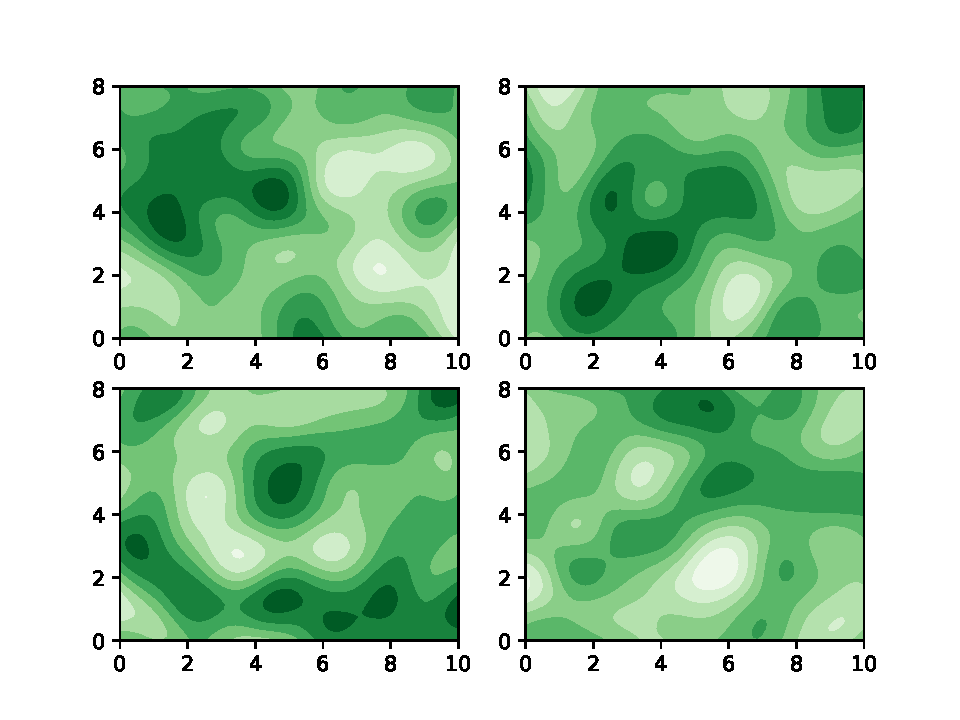
\includegraphics{ellipsoid.files/iso050.pdf}]
Data Sample (kern=0.5)
\end{description}

{]} .pull-right{[}

\begin{description}
\item[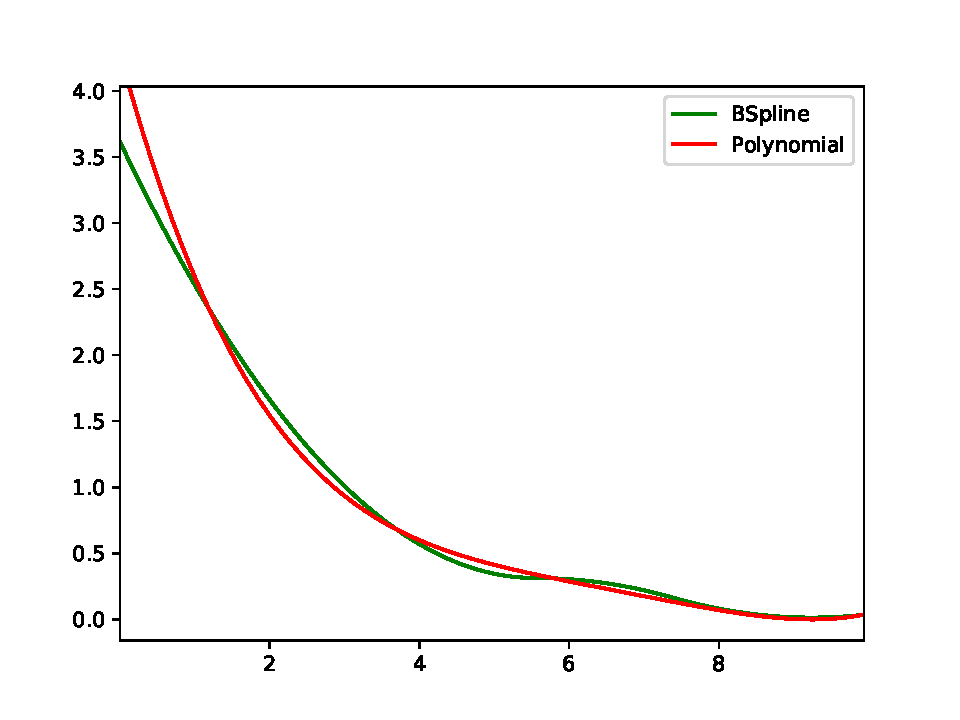
\includegraphics{ellipsoid.files/result050.pdf}]
Least Square Result
\end{description}

{]}

\begin{center}\rule{0.5\linewidth}{0.5pt}\end{center}

\subsection{Experimental Result II}\label{experimental-result-ii}

.pull-left{[}

\begin{description}
\item[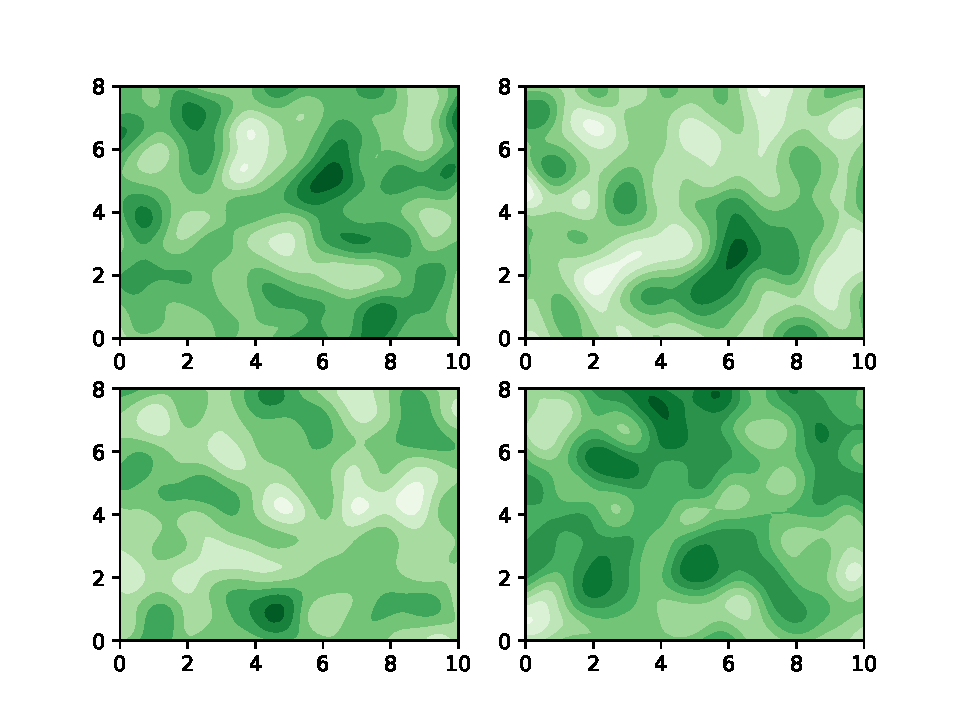
\includegraphics{ellipsoid.files/iso100.pdf}]
Data Sample (kern=1.0)
\end{description}

{]} .pull-right{[}

\begin{description}
\item[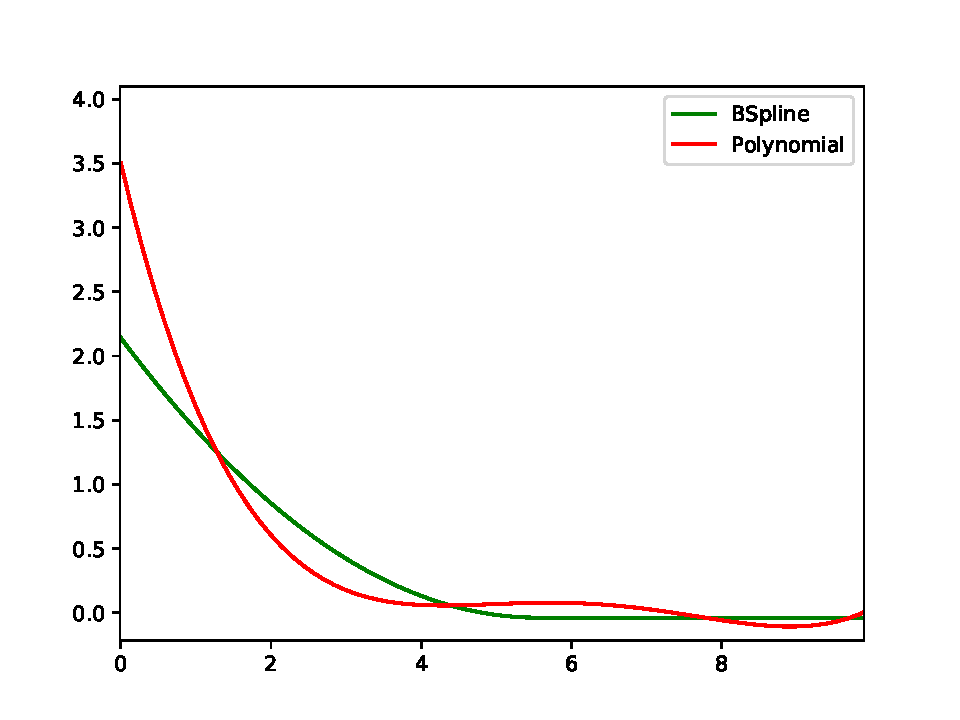
\includegraphics{ellipsoid.files/result100.pdf}]
Least Square Result
\end{description}

{]}

\begin{center}\rule{0.5\linewidth}{0.5pt}\end{center}

\subsection{Experimental Result III}\label{experimental-result-iii}

.pull-left{[}

\begin{description}
\item[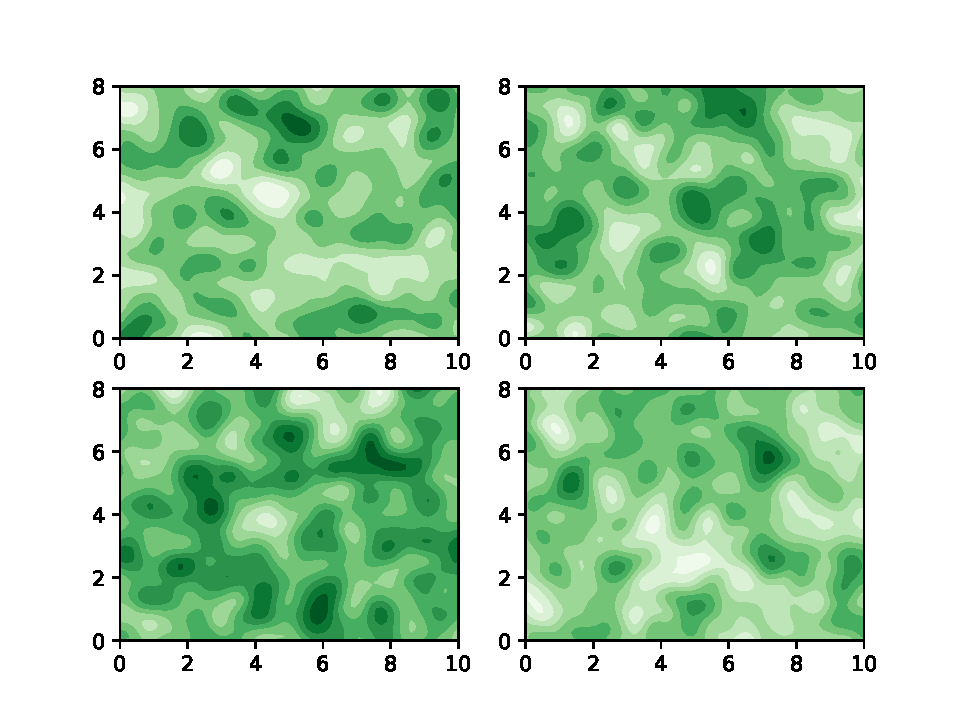
\includegraphics{ellipsoid.files/iso200.pdf}]
Data Sample (kern=2.0)
\end{description}

{]} .pull-right{[}

\begin{description}
\item[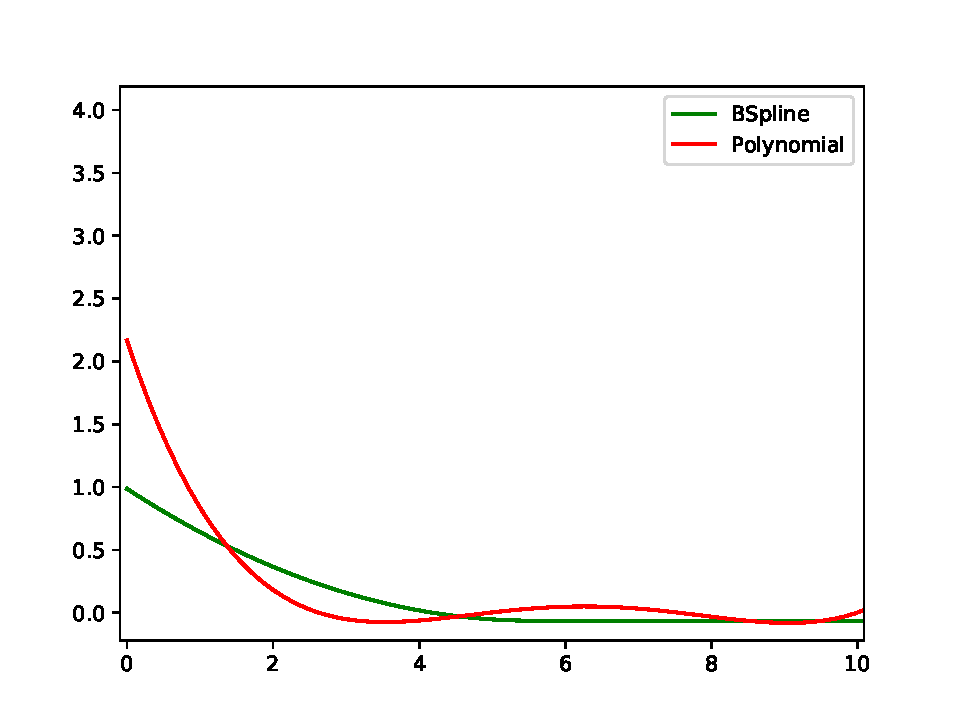
\includegraphics{ellipsoid.files/result200.pdf}]
Least Square Result
\end{description}

{]}

\begin{center}\rule{0.5\linewidth}{0.5pt}\end{center}

class: nord-dark, middle, center

\section{Q \& A}\label{q-a}

\end{document}
